
\documentclass[preprint,review,12pt]{elsarticle}

\usepackage[T1]{fontenc}
\usepackage[utf8]{inputenc}
\usepackage{graphicx}
\usepackage{cellspace}
\usepackage{amsmath}
%\usepackage{cleveref}
%\usepackage{hyperref}
\usepackage{subcaption}
\usepackage{adjustbox}
\usepackage{multirow}
%\usepackage{enumerate}
%\usepackage{mathtools}
\usepackage{algorithm, algpseudocode}

\usepackage{natbib}

\usepackage{lineno,hyperref}
\modulolinenumbers[5]
\usepackage{lipsum}


\journal{Journal of X}

%%%%%%%%%%%%%%%%%%%%%%%
%% Elsevier bibliography styles
%%%%%%%%%%%%%%%%%%%%%%%
%% To change the style, put a % in front of the second line of the current style and
%% remove the % from the second line of the style you would like to use.
%%%%%%%%%%%%%%%%%%%%%%%

%% Numbered
%\bibliographystyle{model1-num-names}

%% Numbered without titles
%\bibliographystyle{model1a-num-names}

%% Harvard
%\bibliographystyle{model2-names.bst}\biboptions{authoryear}

%% Vancouver numbered
%\usepackage{numcompress}\bibliographystyle{model3-num-names}

%% Vancouver name/year
%\usepackage{numcompress}\bibliographystyle{model4-names}\biboptions{authoryear}

% APA style
%\bibliographystyle{model5-names}\biboptions{authoryear}

%% AMA style
%\usepackage{numcompress}\bibliographystyle{model6-num-names}

%% `Elsevier LaTeX' style
\bibliographystyle{elsarticle-num-names}
%%%%%%%%%%%%%%%%%%%%%%%

\begin{document}

\begin{frontmatter}

\title{Coin-Switching Strategy for High-Frequency Trading in Cryptocurrencies Using an Actor-Critic Model and Trend Disentanglement}
%\tnotetext[mytitlenote]{Fully documented templates are available in the elsarticle package on \href{http://www.ctan.org/tex-archive/macros/latex/contrib/elsarticle}{CTAN}.}

%% Group authors per affiliation:
\author{Ahmad Asadi}%\fnref{myfootnote}
\ead{ahmad.asadi@aut.ac.ir}
\author{Reza Safabakhsh\corref{mycorrespondingauthor}}
\cortext[mycorrespondingauthor]{Corresponding author}
\ead{safa@aut.ac.ir}

%\fntext[myfootnote]{Since 1880.}

%%% or include affiliations in footnotes:
%\author[mymainaddress,mysecondaryaddress]{Ahmad Asadi}
%\ead[E-mail]{ahmad.asadi@aut.ac.ir}

%\author[mysecondaryaddress]{Reza Safabakhsh\corref{mycorrespondingauthor}}
%\cortext[mycorrespondingauthor]{Corresponding author}
%\ead{safa@aut.ac.ir}

\address{Deep Learning Lab, Computer Engineering Department}
\address{Amirkabir University of Technology, Tehran, Iran.}

\begin{abstract}
This paper presents a novel framework for cryptocurrency portfolio management, focusing on high-frequency trading (HFT) scenarios, where decisions are made based on predicting near-future trend changes in the asset prices. The framework leverages a Variational Autoencoder (VAE) to disentangle the price behavior of cryptocurrencies into trends and variances, enabling the prediction of trend shifts. A deep reinforcement learning (DRL) model is used to dynamically switch investments between assets, focusing on the single cryptocurrency with the most promising trend at each hour. This coin-switching strategy, in contrast to traditional diversification models, reduces risk while optimizing returns by reallocating investments based on real-time trend predictions. Experimental results show that the proposed model outperforms state-of-the-art strategies in terms of total returns and risk reduction, demonstrating the effectiveness of dynamic coin-switching in volatile markets. Backtesting results on hourly cryptocurrency price data demonstrate that the proposed method achieves more than double the total return on investment compared to baseline strategies, while also reducing maximum drawdowns, highlighting its effectiveness in volatile markets.
\end{abstract}


%%Research highlights
%\begin{highlights}
%	\item A novel uncertainty measurement model for stock price trends is proposed.
%	\item Used disentangled representation learning to find latent factors causing trend shift.
%	\item Used a VAE feature extractor followed by an Actor-Critic for High Frequency Trading.
%	\item Outperformed the baseline models in crypto portfolio management.
%\end{highlights}


\begin{keyword}
	disentangled representation learning \sep
    high frequency trading\sep
    deep reinforcement learning\sep
	stock portfolio management\sep
	variational auto-encoders
	
%\texttt{elsarticle.cls}\sep \LaTeX\sep Elsevier \sep template
%\MSC[2010] 00-01\sep  99-00
\end{keyword}

\end{frontmatter}

\linenumbers

%\section{The Elsevier article class}
%
%\paragraph{Installation} If the document class \emph{elsarticle} is not available on your computer, you can download and install the system package \emph{texlive-publishers} (Linux) or install the \LaTeX\ package \emph{elsarticle} using the package manager of your \TeX\ installation, which is typically \TeX\ Live or Mik\TeX.
%
%\paragraph{Usage} Once the package is properly installed, you can use the document class \emph{elsarticle} to create a manuscript. Please make sure that your manuscript follows the guidelines in the Guide for Authors of the relevant journal. It is not necessary to typeset your manuscript in exactly the same way as an article, unless you are submitting to a camera-ready copy (CRC) journal.
%
%\paragraph{Functionality} The Elsevier article class is based on the standard article class and supports almost all of the functionality of that class. In addition, it features commands and options to format the
%\begin{itemize}
%\item document style
%\item baselineskip
%\item front matter
%\item keywords and MSC codes
%\item theorems, definitions and proofs
%\item lables of enumerations
%\item citation style and labeling.
%\end{itemize}
%
%\section{Front matter}
%
%The author names and affiliations could be formatted in two ways:
%\begin{enumerate}[(1)]
%\item Group the authors per affiliation.
%\item Use footnotes to indicate the affiliations.
%\end{enumerate}
%See the front matter of this document for examples. You are recommended to conform your choice to the journal you are submitting to.
%
%\section{Bibliography styles}
%
%There are various bibliography styles available. You can select the style of your choice in the preamble of this document. These styles are Elsevier styles based on standard styles like Harvard and Vancouver. Please use Bib\TeX\ to generate your bibliography and include DOIs whenever available.
%
%Here are two sample references: \cite{Feynman1963118,Dirac1953888}.



\section{Introduction}
High-frequency trading (HFT) models have revolutionized financial markets, becoming a cornerstone of modern stock and cryptocurrency trading. While traditional HFT focuses on capitalizing on millisecond-level market inefficiencies, a growing body of research highlights the importance of developing models that operate on longer, but still high-resolution, time frames such as hourly intervals. In volatile markets like cryptocurrencies, hourly price movements capture significant trends and reversals, providing opportunities for strategic portfolio adjustments. By leveraging advanced algorithms, real-time analysis, and frequent decision-making, models operating at this granularity can effectively identify short-term price patterns, optimize asset allocation, and enhance portfolio performance. The success of such strategies lies in their ability to respond quickly to evolving market conditions, maximizing returns while mitigating risk over frequent but manageable trading intervals.

A critical aspect of HFT strategies is the prevention of small, cumulative losses, which can have an outsized impact on long-term portfolio performance. Unlike traditional trading, where losses can be balanced over extended periods, HFT operates on razor-thin margins and high transaction volumes, making small losses particularly detrimental. When left unchecked, these losses can compound rapidly, eroding gains and leading to substantial underperformance. Conversely, mitigating minor losses through precise data-driven decision-making can result in exponential returns over time. This dynamic underscores the importance of developing models capable of analyzing micro-level price behaviors and reacting swiftly to unfavorable conditions.

High-frequency trading techniques rely heavily on integrating diverse information sources to identify and capitalize on market trends. Advanced models aggregate technical indicators (\citet{chen2018profitability}), quantitative financial data (\citet{gomber2015high}), crowd-sourced sentiment analysis (\citet{liu2023multi}), and multi-source data fusion approaches (\citet{asadi4423354multi, liu2023multi}). By combining these inputs, HFT models achieve a comprehensive understanding of the market behavior, improving their precision in trend detection and risk mitigation (\citet{li2014online}). This multi-faceted approach empowers traders to not only avoid minor losses, but also uncover critical pivot points in stock price series key moments where trends shift direction. Identifying these pivot points before they occur is central to developing robust strategies capable of maximizing returns while navigating the market's inherent volatility and uncertainty.

While existing research emphasizes the importance of fusing data from multiple sources to identify price series pivot points, we argue that a deeper understanding of price behavior is necessary for predicting trend changes. The ability to anticipate these shifts requires disentangling the factors influencing price movements, such as trend direction and volatility, to predict the probability of changes in the trend of each asset's price in the near future. In highly dynamic markets like cryptocurrencies, even short-term price reversals can significantly impact trading strategies, making it essential to accurately forecast these changes to optimize portfolio performance.

A key innovation of this study is the introduction of a coin-switching strategy that challenges the conventional diversification approach typically employed in portfolio management. Diversification, which involves allocating investments across multiple assets (\citet{markovitz1959portfolio}), is widely used to mitigate risk by reducing dependence on any single asset's performance. However, in high-frequency trading (HFT), where decisions are made at fine-grained time intervals, this traditional approach may not fully exploit opportunities arising from short-term price movements.

In the proposed model, the entire investment value is allocated to a single coin at the start of each investment period, based on the predicted probability of trend shifts for all available coins. This focused strategy enables the model to dynamically select the coin most likely to exhibit a favorable trend, effectively reducing risk while maximizing returns. By disentangling trends and variances for each coin, the model ensures that the selection is data-driven and reflective of the near-term market conditions. Over multiple investment periods, this coin-switching strategy behaves similarly to the cumulative effects of diversification, as the portfolio iteratively adapts to the market's most promising opportunities. Moreover, this approach parallels the concept of concurrent task execution in CPU processing, where tasks are executed in rapid succession to achieve results comparable to parallel computing.

In this paper, we propose a new framework for stock portfolio management that focuses on predicting the probability of near-future trend changes for each asset. The contributions of this study are as follows:

\begin{enumerate}
	\item We introduce a model that disentangles price behavior into meaningful components to predict the likelihood of trend shifts in each asset's price.
	\item We propose a deep reinforcement learning (DRL) model capable of dynamically switching between assets based on the predicted probabilities of trend changes.
	\item We propose a coin-switching strategy for high-frequency trading, where the entire investment is allocated to a single asset during each period. This approach, informed by disentangled trend and variance features, reduces risk while optimizing returns by focusing on the most promising asset at each interval.
	\item The proposed coin-switching method mirrors the cumulative effects of diversification over time by dynamically reallocating investments across assets, akin to concurrent task execution in CPUs.
	\item We demonstrate that the proposed model outperforms state-of-the-art portfolio management strategies in the cryptocurrency market, achieving superior returns and improved portfolio stability.
\end{enumerate}

By leveraging disentangled price features, reinforcement learning, and innovative allocation strategies, the proposed framework addresses the challenges of frequent decision-making in dynamic financial markets and enhances the ability to adapt to near-term price trends.

The rest of this paper is organized as follows: In Section 2 we review the existing models for stock portfolio management and stock price trend predictors. Section 3 describes in detail the structures of the time-series uncertainty estimation model and the deep reinforcement learning model. The proposed model is then evaluated and the results are reported and discussed in Section 4. Finally, the conclusions of the paper are summarized in Section 5.
\section{Related Work}
In general, portfolio management studies can be categorized into the following closely related areas: Portfolio Optimization, Portfolio Allocation, and Portfolio Selection \cite{ozbayoglu2020deep}. Meanwhile, asset pricing models that aim to predict the future prices of stocks and derivatives in financial markets are also common approaches that help portfolio management models to propose portfolio vectors based on the predicted prices \cite{nazareth2023financial}.
\subsection{Information Fusion in Stock Portfolio Management}

The use of deep learning models in stock portfolio management is very well justified due to their ability to process vast amounts of data and extract complex patterns that traditional models may overlook. Traditional portfolio management strategies often rely on statistical models (\citet{li2012pamr}) and optimization models (\citet{pennanen2012introduction}) to make investment decisions. However, with the advent of deep learning and deep reinforcement learning techniques, researchers and practitioners have started exploring more sophisticated and data-driven approaches mostly based on using technical indicators to portfolio management (\citet{ayala2021technical}, \citet{agrawal2022stock}, \citet{taghian2021reinforcement}, and \citet{taghian2022learning}).

Due to the capabilities of deep learning models in financial markets specially their abilities to process large amounts of complex data, the fusion of various types of information plays a crucial role in enhancing the performance of deep learning-based portfolio management systems. One common approach to information fusion in deep learning-based stock portfolio management is the use of multi-modal data inputs (\citet{asadi4423354multi}). This involves combining different types of data, such as historical price data, financial statements, news sentiment, and social media feeds, into a single model. By incorporating multiple modalities of information, these models can capture a more comprehensive view of market dynamics and make more informed investment decisions.

Another approach to information fusion is the use of ensemble methods, where multiple deep learning models are trained on different subsets of data or with different architectures (\citet{carta2021multi}). The outputs of these models are then combined to generate a consensus prediction, which can be more robust and accurate than any individual model. \citet{lin2022multiagent} proposed a deep reinforcement learning (DRL) based model with multiple agents and designed a long-term reward function to reduce the risk of investment with fusing the decisions of different agents. \citet{hao2023stock} proposed a three-dimensional fuzzy representation of stock price trend and employed an ensemble DRL model for stock portfolio management based on the fuzzy representation of the price trend.

Furthermore, attention mechanisms have been proposed as a way to selectively focus on relevant information within a dataset, specifically in gathering information from multiple markets (\citet{zhao2022stock}). Another important deep learning model which is used for fusing temporal information for stock portfolio management is the Transformers model (\citet{gullotto2021portfolio}). \citet{kisiel2022portfolio} proposed a deep learning model based on a transformer for minimizing the small losses of stock trading with optimizing the Sharpe ratio \citet{sharpe1998sharpe} directly. \citet{liu2023revolutionising} combined a non-stationary transformer model with a DRL model for fusing macro-economic information with targeted news sentiments.

%Overall, the survey of different approaches to information fusion in deep learning-based stock portfolio management highlights the importance of integrating diverse sources of data and leveraging advanced techniques to enhance performance and robustness. By combining multiple modalities, using ensemble methods, and incorporating attention mechanisms, researchers and practitioners can develop more sophisticated and effective models for managing stock portfolios in dynamic financial markets.
%
%
%Deep reinforcement learning (DRL) is another area of interest in stock portfolio management, as it enables the development of dynamic trading strategies that adapt to changing market conditions. DRL algorithms, such as the Deep Q-Network (DQN) and Proximal Policy Optimization (PPO), have been utilized to train agents to make buy/sell decisions based on market signals and portfolio performance metrics. These models can learn optimal trading policies through trial-and-error interactions with the market environment, leading to potentially more robust and adaptive portfolio management strategies.


\subsection{Uncertainty Measurements in Stock Trading Strategies}

Uncertainty is a fundamental aspect of financial markets, and accurately measuring and managing uncertainty is crucial for developing effective stock trading strategies. In recent years, researchers have focused on exploring various methods and metrics to quantify uncertainty in stock trading, with the aim of improving decision-making processes and reducing risk exposure. This literature review provides an overview of the key studies and approaches related to uncertainty measurements in stock trading strategies (\citet{abdar2021review}).


The first category of models proposed for portfolio management with considering the risk of investment, are those that try to minimize investment risk by diversification of the proposed portfolios. \citet{du2022mean} proposed a mean-variance portfolio proposition based on the co-integrated stocks and their correlation. 

Considering risk-related measures for optimizing deep learning model weights is another approach in which the trained model would consider the uncertainty of the stock prices in portfolio proposition. \citet{syu2020portfolio} proposed a DRL based model in which the Sharpe ratio of portfolio proposals is used to optimize the model weights.

A novel model recently introduced by \citet{abdulsahib2024cross} in this field utilizes disentangled representation learning to break down the input features from various markets and identify the common factors during the representation learning phase. By decomposing the features of distinct markets and identifying shared features between them, the model can better understand the interconnected dynamics between the markets and predict price movements in one market based on the behavior of shared features with another market. Furthermore, the concept of disentangled representation learning was previously employed by \citet{abdulsahib2023glad} to study the price dynamics of stocks in financial markets.


While most of related work has focused on integrating information from various sources in stock portfolio management, this study seeks to break down the fundamental factors that influence price behavior. The goal is to detect indications of trend changes and identify price pivot points before they occur. To achieve this, disentangled representation learning is utilized to create a latent space based on historical stock price data, where latent features indicate potential price changes. A feature extractor is developed to detect price pivot points, and an actor-critic model is proposed to pinpoint the optimal time to switch between stocks to mitigate losses.

\section{Proposed Method}
The model proposed in this paper consists of two modules. The first module is a feature extractor which is enabled to extract features indicating the strength of the current price trend in the near future. The second module is an actor-critic based model which selects a single coin to buy and hold until the next investment interval based on the uncertainty about the price trends of each coin extracted by the first module. 

Figure \ref{fig:arch} illustrates the architecture of the model presented in this study. The model is built on the concept of disentangled representation learning, where a feature extractor is trained to extract features from the historical price data of each coin. These extracted features are then combined and fed into an actor-critic model to select a single coin from the available options in the market. It is important to note that the portfolio proposals in this research consist of only one coin, and no combinations of coins are considered. This constraint is imposed to enhance the clarity of the model's investigation and facilitate comparisons with the existing models in the field.


%In the context of stock trading, we approach the complex task by decomposing it into two distinct components: leveraging pre-trained deep learning models for portfolio management as expert models, and introducing a novel Model Switching Agent (MS Agent) designed to dynamically select the most suitable expert model based on the current state of the environment and the performance of each expert model. This two-pronged approach aims to enhance the adaptability and effectiveness of the overall trading system by intelligently switching between expert models to optimize decision-making in response to changing market conditions. Figure \ref{fig:arch} illustrates the structure of this idea.

\begin{figure}[H]
	\centering
	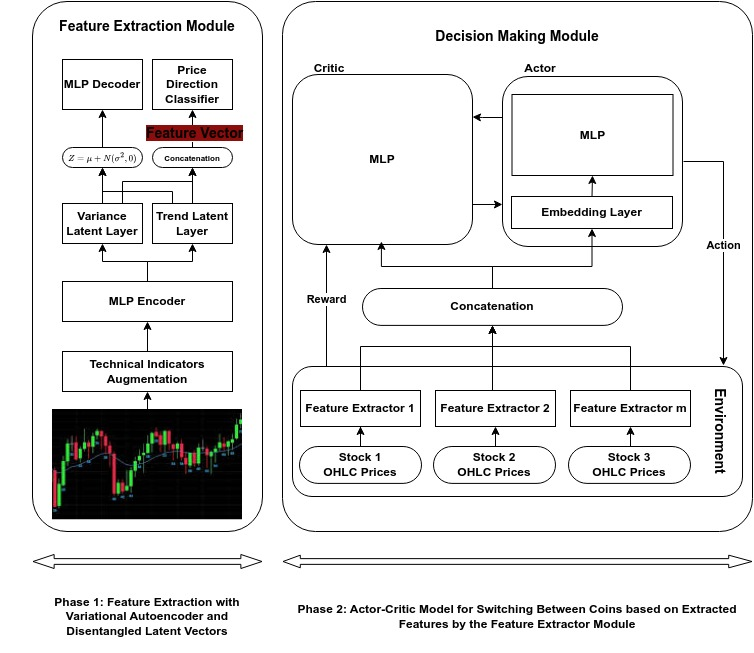
\includegraphics[scale=0.6]{./NewArch.jpg}
	\caption{The structure of Model Switching idea for stock trading}
	\label{fig:arch}
\end{figure}


\subsection{Feature Extraction}

Disentangled representation learning is a powerful technique in machine learning that aims to learn representations of data where different factors of variation are separated into distinct and interpretable components. This can be particularly useful in time series data, where multiple underlying processes may be present and need to be disentangled for better understanding and analysis.

Let's consider a time series dataset $X = \{x^1, x^2, ..., x^t\}$, where $x^i$ represents the observation at time step $i$. The goal of disentangled representation learning on time series is to learn a set of latent variables $Z = \{z_1, z_2, ..., z_K\}$ that capture the underlying factors of variation in the data. These latent variables should be disentangled, meaning that each $z_k$ represents a different aspect of the data that is independent of the others.

Given the assumption of independence among the generating factors, the task of disentangled representation learning in a dimension-wise manner aims to encode the information pertaining to these generating factors by means of a latent vector of lower dimensionality - as a compact representation of the high-dimensional observations. The relationship between the observations and the latent vectors can be formally characterized by their joint distribution

\begin{align}
	p_\theta(x,z) &= p_\theta(x|z) p_\theta(z) \label{eq:1}\\
	p_\theta(z) &= N(z|0, \sigma^2 I) \label{eq:2}
\end{align}

where $\theta$ denotes the set of parameters of the feature extractor model and the prior distribution $p(z)$ is typically assumed to be a multidimensional Gaussian distribution with the same variance in all directions 


One common approach to achieve disentangled representation learning on time series data is through Variational Autoencoders (VAEs) (\citet{duan2019unsupervised}, \citet{li2022towards}, and \citet{li2021learning}). VAEs are generative models that learn a probabilistic mapping between the observed data and the latent variables. By introducing a prior distribution over the latent variables, VAEs can learn disentangled representations by encouraging the latent variables to capture independent factors of variation in the data.

In the first module of the proposed method, we utilize a VAE structure to capture the underlying distribution of the data and extract disentangled representations for uncertainty measurement in stock portfolio management. The VAE is designed to learn a latent space that separates different factors of variation in the data, enabling us to better understand and quantify the uncertainty associated with our model's predictions.

The VAE consists of an encoder network that maps input data (e.g., historical stock prices, market indicators) to a latent space representation, and a decoder network that reconstructs the input data from the latent space. By training the VAE to minimize the reconstruction error and maximize the mutual information between the input and latent representations, we aim to learn a compact and meaningful representation of the data that facilitates uncertainty estimation.

To encourage disentangled representation learning in the VAE, we incorporate regularization techniques, such as $\beta$-VAE (\citet{burgess2018understanding}) or disentanglement loss functions, that promote the separation of different factors of variation (e.g., market trends, individual stock performance) in the latent space. This disentangled representation enables us to measure uncertainty more effectively and make informed decisions in stock portfolio management.

The relation between the latent features and input data in the proposed VAE model is described in equation \eqref{eq:beta-vae}.

\begin{equation}
	z_i = \hat{\mu_i} + \hat{\sigma_i} \epsilon
	\label{eq:beta-vae}
\end{equation}

where $z_i$ denotes the $i$th element of the latent vector, $\hat{\mu_i}$ and $\hat{\sigma_i}$ respectively represent the latent vectors learned by the encoder to simulate the mean and variance of the price series, and $\epsilon \propto N(0, 1)$ denotes a random white noise.

Since the latent vectors $\hat{\mu_i}$ and $\hat{\sigma_i}$ are the vectors that are passed to the portfolio manager module, they are assumed to encode information regarding price trend. In addition, these vectors should be informative enough to estimate our uncertainty about the persistence of the current price trend in the near future. Therefore, a classifier is embedded inside the VAE model and an extra term is added to VAE model's loss function to ensure that $\hat{\mu_i}$ and $\hat{\sigma_i}$ encode necessary information.

A binary classifier $\Phi(\hat{\mu}, \hat{\sigma})$ is augmented into the VAE model in order to enforce latent variables to encode information related to future price trend. The ground-truth labels for this classifier are generated via equation \eqref{eq:class1}.
\begin{equation}
	Y_i^t = 
	\begin{cases}
	\text{1} &\quad\text{if } \frac{x_i^{t+l}}{x_i^t} > 1\\
	\text{-1} &\quad\text{otherwise}
	\end{cases}
	\label{eq:class1}
\end{equation}

where $\frac{x_i^{t+l}}{x_i^t}$ computes the total return of stock $i$ in $l$ steps ahead from time step $t$ and $Y_i^t$ denotes the label of the classifier for stock $i$ in time step $t$. Based on equation \eqref{eq:class1}, the proposed loss function for learning the set of parameters of the VAE model is presented in equation \eqref{eq:lossVAE}.
\begin{align}
	\mathcal{L} &= \mathcal{E}  + \mathcal{C} - \mathcal{K}	\label{eq:lossVAE}  \\
	\mathcal{E} &= \Sigma_{i=1}^S \Sigma_{t=w}^T (\hat{X_i^t} - X_i^T) ^ 2 	\label{eq:lossVAE2} \\
	\mathcal{C} &= \Sigma_{i=1}^S \Sigma_{t=w}^T \Gamma(\Phi(\hat{\mu_i^t}, \hat{\sigma_i^t}), Y_i^t) 	\label{eq:lossVAE3} \\
	\mathcal{K} &= \frac{1}{2} \Sigma_{i=1}^S \Sigma_{t=w}^T (1 + log(\hat{\sigma_i^t})^2 - \hat{\mu_i^t}^2 - (\hat{\sigma_i^t})^2 	\label{eq:lossVAE1} 
\end{align}
where the loss function $\mathcal{L}$ for the VAE model is decomposed into three distinct components: $\mathcal{E}$ for reconstruction loss, $\mathcal{K}$ for Kullback-Leibler divergence, and $\mathcal{C}$ for the classification loss. Moreover, the variables $w$, $S$ and $T$ represent the window size, the number of stocks in the dataset, and the maximum time-step in the training set, respectively.

The VAE model undergoes training separately from the other components of the proposed model. The dataset necessary for training the VAE model comprises time-series data of stock historical prices divided into windows of size $w$, with the corresponding labels based on equation \eqref{eq:class1}.

\subsubsection{Stock Switching}

In the second part of our method, we propose an Actor-Critic neural network architecture for generating optimal stock portfolios over a set of liquid coins in the cryptocurrencies market. The Actor network learns a policy that selects one of the available stocks based on the current state of the market and the uncertainty estimates on current price trend of each stock provided by the VAE. The Critic network evaluates the value of the chosen actions and provides feedback to update the policy.

The Actor-Critic architecture leverages reinforcement learning techniques to optimize the stock portfolio management strategy over time, taking into account both immediate rewards (e.g., profit/loss) and long-term objectives (e.g., investment risk and returns in long run). By incorporating uncertainty measurements from the VAE into the decision-making process, our model can adapt to changing market conditions and make more robust portfolio recommendations.

Overall, our method combines disentangled representation learning with deep reinforcement learning to enhance stock portfolio management by effectively measuring uncertainty and optimizing portfolio decisions in the volatile cryptocurrencies market. Through this integrated approach, we aim to improve the performance, stability, and interpretability of AI-driven investment strategies for financial applications.

The Actor network is designed to generate actions based on the input data. It consists of two fully connected layers with LeakyReLU activation functions to introduce non-linearity and facilitate learning complex patterns. The final layer of the Actor network is a Softmax layer, which normalizes the output values into a probability distribution over the available actions. This distribution determines the action to be taken at each time step.

The Critic network is responsible for evaluating the actions generated by the Actor network. It consists of two fully connected layers, similar to the Actor network. However, the last layer of the Critic network contains only one node, which outputs a scalar value representing the estimated return associated with the generated action. The Critic network utilizes a logarithmic estimate of the return values as its reward function, providing a measure of the quality of the actions taken by the Actor network.

The overall structure of the Actor-Critic model is illustrated in Figure \ref{fig:arch}. The Actor network generates actions based on the input data, while the Critic network evaluates these actions to provide feedback to the Actor network. This feedback loop enables the model to learn and improve its trading strategies over time.


In addition, a novel immediate reward function is proposed. It calculates the difference between the immediate return of the model's proposed action and the optimal return achievable based on future prices of each coin. This reward function is defined by Equation \eqref{eq:ri}.
\begin{equation}
	\mathcal{R}_t = log(\frac{1}{1 + [\Sigma_{j} a_j^t * R_j^t] - max_j(R_j^t)})
	\label{eq:ri}
\end{equation}
where $\mathcal{R}_t$ denotes the immediate reward of the stock switching agent at time step $t$, $R^t = \{r_1^t, \cdots, r_n^t\}$ is the set of stock returns in which $r_i^t = \frac{X_i^{t+1}}{X_i^t}$ represents the next time-step return of stock $i$, and the $j$th element of the action vector at time step $t$ is denoted by $a_j^t$. The best immediate stock return is calculated as $max_j(R_j^t)$ and the return of the agent's action is computed as $ [\Sigma_{j} a_j^t * R_j^t]$. If the agent selects the best stock at time-step $t$, the difference between the action return and the best stock return is zero; otherwise, it is a negative value greater than $-1$. Equation \eqref{eq:ri} suggests that the maximum reward is attained when there is no difference between the agent's selection and the best stock.
\section{Experimental Results}
%\lipsum[2]

\subsection{The Dataset}

In our study, we analyze a dataset consisting of historical daily OHLC (Open, High, Low, Close) data for the ten most liquid crypto-currencies in the market over the recent years\footnote{The OHLC prices were collected using the "CoinGeckoAPI" in Python. For more information, visit \url{https://www.coingecko.com/en/api}}. The coins chosen for our research are listed in Table \ref{tbl:data} . It is important to note that in cases where a coin has fewer than 3838 days of price data, the price series is extended by repeating the initial data point to fill the time interval.

\begin{table}[h]
	\centering
	\caption{List of selected coins in experimental data-set}
	\begin{tabular}{c|c|c|c}
		Symbol & Start Date & End Date & Number of available daily records \\
		\hline
		\hline
		bitcoin & 2013-04-29 & 2023-11-01& 3838 \\
		ethereum & 2015-08-07 & 2023-11-01& 3008 \\
		binancecoin & 2017-09-17 & 2023-11-01& 2236 \\
		binance-peg-xrp & 2021-05-12 & 2023-11-01& 903 \\
		solana & 2020-04-10 & 2023-11-01& 1300 \\
		litecoin & 2013-04-29 & 2023-11-01& 3838 \\
		binance-peg-polkadot & 2021-05-12 & 2023-11-01& 903 \\
		binance-peg-cardano & 2021-05-12 & 2023-11-01& 903 \\
		dogecoin & 2013-12-17  & 2023-11-01& 3606 \\
		matic-network & 2019-04-26 & 2023-11-01& 1650\\
		
	\end{tabular}
	\label{tbl:data}

\end{table}

This dataset provides a comprehensive view of the price movements and trends in the crypto market, enabling us to evaluate the performance of the proposed method for stock portfolio management under real-world conditions. Figure \ref{fig:dataset} illustrates 100 random price series available in the dataset.

\begin{figure}[h]
	\centering
	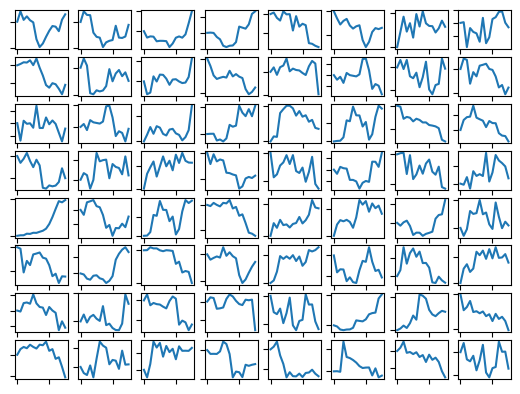
\includegraphics[scale=0.8]{./dataset.png}
	\caption{Sample coin price time-series from the available dataset.}
	\label{fig:dataset}
\end{figure}

In the rest of this section we will investigate different aspects of the proposed model in portfolio management. Section 4.2 studies the features of the latent space learned by the VAE model. Section 4.3 provides an ablation study on the proposed model and a makes a comparison between the performance of different versions of the proposed model. Section 4.4 compares the results of the proposed model with the baseline models.

\subsection{Latent Space Investigation}

The primary goal of the proposed model is to establish a suitable framework for quantifying the uncertainty surrounding the persistence of the prevailing stock price trend, with the aim of identifying the underlying rationale for adjusting portfolio assets based on forecasts of future price movements for individual stocks. The proposed VAE model outlined in Section 3.1 is tasked with capturing a latent space from the input price time-series data to assess the likelihood of a shift in trend direction in the future. Consequently, an examination of the characteristics of the acquired latent space within this model can offer insights into the efficacy of the proposed approach and its overarching objective.

To facilitate a clearer examination of the latent space and to shift the emphasis towards analyzing the model's behavior within this learned space, we investigate the model's performance using a synthetic dataset comprising noisy sine waves. Given that the concept of \textit{"mean reversion"}\footnote{Mean reversion is a statistical property observed in financial markets where stock prices tend to fluctuate around a long-term average, with extreme price movements typically followed by a corrective movement that brings the price closer to its historical mean. For more information about reports investigating mean reversion property in financial markets refer to \citet{enow2023investigating} and \citet{corbet2020asymmetric}.} is commonly utilized in the analysis of financial time series, we opt for a dataset featuring noisy sine waves due to their simplistic structure and resemblance to financial time series exhibiting mean reversion over extended periods.

The synthesized series in this tiny dataset are generated based on the equation \eqref{eq:sines}.
\begin{equation}
	\zeta_t^i = \epsilon_t + sin(\nu^i + \frac{t}{2\pi})
	\label{eq:sines}
\end{equation}
where $\zeta_t^i$  represents the $t$th element in the $i$th time series within the generated dataset. White noise $\epsilon_t \propto N(0,1)$ is introduced at each time step to add noise to the generated sequences, and a random uniform offset  $\nu^i \propto U(0, 2\pi)$ is applied to the $i$th sample in the dataset. Random windows based on equation \eqref{eq:sines} are generated and labeled using equation \eqref{eq:class1}. The VAE model is trained using the synthetic time series dataset. Given that all input samples in the generated dataset consist of sequences of scalar values, the model assumes the cardinality of both latent features are set to 1.

Figure \ref{fig:latent_sine} demonstrates the VAE's generation of random samples with varying $\hat{\mu}$ and $\hat{\sigma}$. The illustration involves traversing the latent space while adjusting $\hat{\mu}$ and $\hat{\sigma}$ values from $-1$ to $+1$. The top left image corresponds to $\hat{\mu} = -1$ and  $\hat{\sigma} = -1$, the top right image to $\hat{\mu} = +1$ and  $\hat{\sigma} = -1$, the bottom left image to $\hat{\mu} = -1$ and  $\hat{\sigma} = +1$, and the bottom right image to $\hat{\mu} = +1$ and  $\hat{\sigma} = +1$.

Figure \ref{fig:latent_sine} highlights two key aspects. First, the VAE model effectively learns to separate data based on the series trend within the latent space. Samples near the center of the space, around $\hat{\mu} = 0$ and  $\hat{\sigma} = 0$, exhibit a subtle change in price trend, whereas those in the corners display a clear and distinct trend. Second, the latent space is populated with quarters of sine series that exhibit transitions in trend at their beginnings or endings. This indicates that the proposed VAE model can differentiate factors associated with price changes by leveraging its classification loss to disentangle the latent space effectively.

\begin{figure}[h]
	\centering
	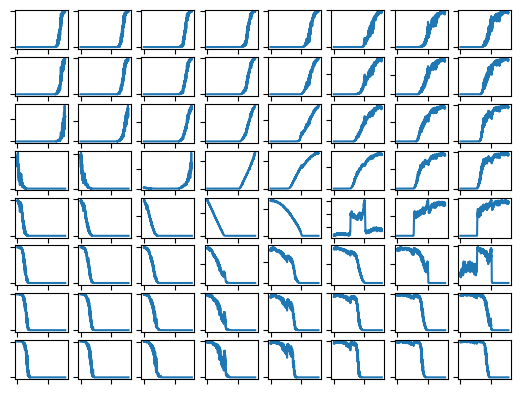
\includegraphics[scale=0.8]{./model_latent_sine.png}
	\caption{Illustration of the latent space learned by simple VAE over noisy sine series.}
	\label{fig:latent_sine}
\end{figure}

In the next experiment, the VAE model was trained using the closing price sequences from the crypto-currency dataset. Similarly, both latent features were constrained to a cardinality of $1$ for this experiment. The latent space generated from this training is visualized in Figure \ref{fig:latent_full}. The series displayed in the upper section of the figure represent series with consistently positive price trend, whereas those in the lower section depict abrupt declines. This visualization effectively demonstrates the VAE model's ability to disentangle distinct trends within the data.


%
%\begin{figure}[h]
%\centering
%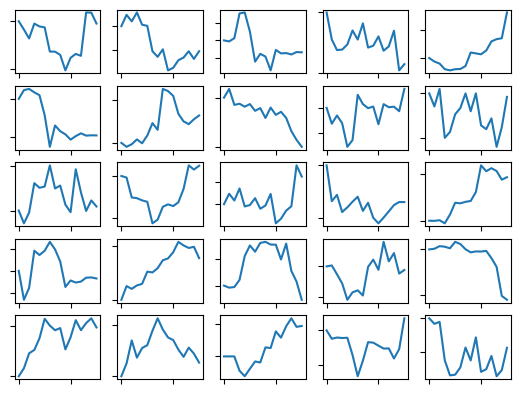
\includegraphics[scale=0.8]{./model_latent_space_wo_classifier.png}
%\caption{Illustration of the latent space learned by simple VAE over model performance series.}
%\label{fig:latent_wo_classifier}
%\end{figure}


\begin{figure}[h]
	\centering
	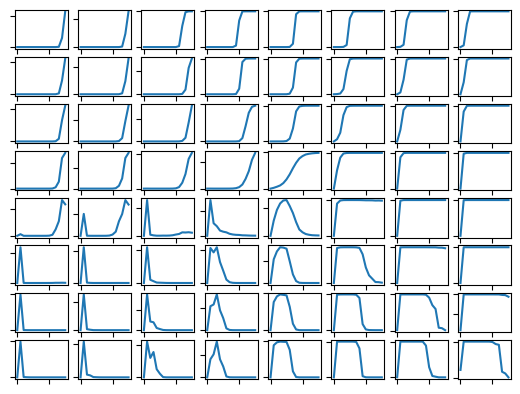
\includegraphics[scale=0.8]{./model_latent_space.png}
	\caption{Illustration of the latent space learned by VAE with classifier over model performance series}
	\label{fig:latent_full}
\end{figure}


\subsection{Ablation Study}

To assess the effectiveness of different components of the proposed method, we conduct an ablation study where we systematically analyze the impact of key elements such as the VAE for uncertainty measurement and the Actor-Critic neural network for stock portfolio proposal. By comparing the performance of the complete model with variations that exclude specific components, we aim to understand the contribution of each part to the overall coin switching strategy.

\subsubsection{Feature Extraction}
In the initial experiment in ablation study, our objective is to examine the influence of the VAE model on classification of price trend movement direction. For this aim, we utilize a multi-layer perceptron (MLP) network to categorize the direction of price movements based on the definition outlined in equation \eqref{eq:class1}. The outcomes of price trend prediction using various classifiers are compared in Table \ref{tbl:FE-pred}.

The baseline models considered in this study are as follows:
\begin{itemize}
	\item \textbf{MLP}. This model is a basic MLP classifier trained directly on the input series without any feature extraction.
	\item \textbf{VAE-Z}. Here, the VAE is trained, and only the embedding vector $Z$ is provided to the classifier as the extracted feature.
	\item \textbf{VAE-TR}. In this model, the VAE is trained, and the concatenated latent vectors $\hat{\mu}$ and $\hat{\sigma}$ are passed to the classifier as the extracted feature.
	\item \textbf{VAE-Y}. This model involves training the VAE, and only the VAE's embedded classifier output $\hat{Y} = \Phi(\hat{\mu}, \hat{\sigma})$ is used as the extracted feature.
	\item \textbf{VAE-FULL}. In this setup, the VAE is trained, and all encoder outputs containing $Z$, $\hat{\mu}$, and $\hat{\sigma}$ are concatenated and provided to the classifier as the extracted feature.
\end{itemize}

Table \ref{tbl:FE-pred} presents a comparison of the baseline models' accuracy in the classification task. The results indicate that model \textbf{VAE-Y} performs the best as a feature extractor. This observation supports our hypothesis that accurately predicting the likelihood of continuation of the current stock price trend can assist portfolio management models in determining optimal points for asset switching within the portfolio.

\begin{table}[h]
	\centering
	\caption{Comparison between baseline models accuracy in predicting the future price trend direction}
	\label{tbl:FE-pred}
	\begin{tabular}{c | c | c | c | c | c }
		Method & MLP & VAE-Z & VAE-TR & VAE-Y & VAE-FULL \\
		\hline
		\hline
		Train & 63.48& 76.94 & 95.36 & \textbf{95.45} & 94.36\\
		Test & 61.80& 73.59 & 93.47 & \textbf{95.55} & 94.72\\
	\end{tabular}
\end{table}

\subsubsection{Latent Space Dimensionality}
The following experiment aims to explore how the size of latent vectors $\hat{\mu}$ and $\hat{\sigma}$ influences the quality of extracted features. In this study, we varied the dimensions of the latent vectors and assessed the classifier's accuracy in predicting the next price movement direction.

The comparison of these models is presented in Table \ref{tbl:FE-dim}. The findings from this table suggest that enhancing the dimensionality of latent vectors leads to improved model performance. This improvement can be attributed to the larger latent vector size enabling the model to more effectively encapsulate the extracted information into a single vector. It is worth noting that as the dimensionality increases, more data is required for training, and therefore, performance gains may plateau after reaching a certain threshold with a fixed dataset size.


\begin{table}[h]
	\centering
	\caption{The impact of the latent vectors size on the accuracy of the price trend prediction}
	\label{tbl:FE-dim}
	\begin{tabular}{c | c | c | c | c | c }
		Method & 1 & 10 & 50 & 150 & 200 \\
		\hline
		\hline
		Train & 95.45& 96.02 & 98.51 & \textbf{98.85} & 95.46\\
		Test & 95.55& 94.16 & 97.37 & \textbf{98.23} & 91.24\\
	\end{tabular}
\end{table}

\subsubsection{Reward Function}
The reward function proposed for the coin-switching agent in equation \ref{eq:ri} is designed based on the distance between the selected coin by the agent and the best coin at each time step. This approach aims to incentivize the agent to learn to switch to the best coin at every time step. Another commonly used reward function in this research domain is the total portfolio return at each time step. To evaluate the effectiveness of the proposed reward function, a comparison between these two models is presented in table \ref{tbl:rewards}. The table includes metrics such as total return on investment (\textbf{total-ROI}), maximum drawdown (\textbf{MDD}), and average return (\textbf{AR}) for each model. The results indicate that the model utilizing the proposed return function demonstrates superior performance compared to the traditional reward function commonly used in the field.


\begin{table}[h]
	\centering
	\caption{The impact of proposed reward function}
	\label{tbl:rewards}
	\begin{tabular}{c | c | c | c  }
		Method & total-ROI & MDD & AR \\
		\hline
		\hline
		Proposed Reward & \textbf{125 \%}  & \textbf{-19 \%} & \textbf{0.27}  \% \\
		Common Reward & 54 \%  & -20 \%  & 0.15 \%\\
	\end{tabular}
\end{table}


\subsubsection{Considering Risk-free Asset}
One of the main underlying assumptions in our study was that mitigating minor losses would enhance portfolio management effectiveness. Consequently, we conducted an additional experiment to investigate how our model performs with and without the inclusion of a risk-free asset. Table \ref{tbl:rf1} presents a comparison of the model's performance under these conditions. The results indicate that the model performs better when the risk-free asset is included, particularly in terms of metrics such as maximum drawdown. This suggests that timely switching to the risk-free asset can help prevent losses in the investment process.

\begin{table}[h]
	\centering
	\caption{The impact of risk-free asset presence on model's performance}
	\label{tbl:rf1}
	\begin{tabular}{c | c | c | c  }
		Method & total-ROI & MDD & AR \\
		\hline
		\hline
		with tether & \textbf{125 \%}  & \textbf{-19 \%} & \textbf{0.27}  \% \\
		without tether & 28 \% & -34 \% & 0.11 \% \\
	\end{tabular}
\end{table}

%To demonstrate the efficiency of the proposed model in identifying and transitioning to the risk-free asset at opportune moments, we conducted an additional experiment. In this study, we defined periods where all coins exhibited a bearish price trend as bearish markets, with all other times classified as bullish. Subsequently, we evaluated the behavior of the coin-switching agent in terms of its ability to switch to the risk-free asset during bearish market conditions. The outcomes of this experiment are presented in Table \ref{tbl:rf2}. The true positive metric (TP) signifies the percentage of instances where the coin-switching agent correctly switched to the risk-free asset, while the false positive metric (FP) indicates the percentage of incorrect switches, and so forth. The results reveal that in the presence of a risk-free asset, the model effectively learns to transition to this asset when the majority of other coins are experiencing a bearish price trend. Our findings demonstrate that the coin-switching agent successfully switched to the risk-free asset in approximately 30\% of instances when all available coins were in a bearish trend.
%
%\begin{table}[h]
%	\centering
%	\caption{The confusion matrix of the proposed model indicating the power of the model in switching to the risk-free asset at proper times.}
%	\label{tbl:rf2}
%	\begin{tabular}{c | c | c }
%		Market & Positive & Negative \\
%		\hline
%		\hline
%		Positive & 0& 0 \\
%		Negative & 0& 0 \\
%	\end{tabular}
%\end{table}

%The experiment's results is summarized to compare various iterations of the proposed model. Table \ref{tbl:cmp1} presents the performance metrics of these models for comparison. The findings from the table indicate that the model utilizing \textbf{VAE-Y} as the feature extractor and incorporating the suggested reward function that accounts for the risk-free asset outperforms other versions of the model.

\subsection{Portfolio Proposals}
The primary objective of the proposed model is to identify optimal time points for transitioning between different coins in the market. While the model's primary focus is distinct from portfolio management in which models are supposed to propose a combination of instruments at each time-step, we conducted a performance evaluation by comparing it against both single asset trading strategies and portfolio management models to assess its effectiveness in identifying optimal transition points between coins.

\subsubsection{Baselines}
The baseline models that have been compared with the proposed model are outlined below:

\begin{itemize}
	\item \textbf{BaH(X)}. This denotes the buy and hold strategy, where coin X is purchased at the beginning of the experiment and held until the end.
%	\item \textbf{MLP-vanilla} \citet{taghian2022learning}.  This model, introduced by \citet{taghian2022learning}, involves a Deep Reinforcement Learning (DRL) model that learns candlestick patterns and establishes generalized trading rules for Bitcoin.
	\item \textbf{UCRP}. Uniform Constant Rebalanced Portfolio strategy involves setting the portfolio proposal vector to a uniform vector $w^t=(\frac{1}{n}, \cdots, \frac{1}{n})$ at the start of each time step, where $n$ represents the number of available coins and $|w^t| = n$.	
	\item \textbf{FTW}. Following the winner strategy adjusts the portfolio proposal vector at each time step based on the historical performance of coins, with weights of winning coins revised according to their cumulative return $w^t = SoftMax(CR_t)$, where $CR_t$ calculated as in equation \eqref{eq:ftw}.
	\begin{align}
		CR_t = \{R(X_i^{1:t})| \> &X_i^{1:t} = \{X_i^1, \cdots, X_i^t\} \> \land  \notag \\ 
		&R(X_i^{1:t}) = \frac{X_i^t}{X_i^1} \> \land \notag \\ 
		&i \in \{1, \cdots, n\}\}
		\label{eq:ftw}
	\end{align}

	\item \textbf{FTL}. Following the loser strategy refines the portfolio proposal vector at the beginning of each time step by adjusting the weights of losing coins based on the inverse of their historical performance $w^t = SoftMax(CR_t^{-1})$, using $CR_t^{-1}$ computed as shown in equation \eqref{eq:ftl}.
	\begin{align}
	CR_t^{-1} = \{R(X_i^{1:t})^{-1} | &X_i^{1:t} = \{X_i^1, \cdots, X_i^t\} \> \land \notag\\ 
	&R(X_i^{1:t})^{-1} = \frac{1}{1 + log(\frac{X_i^t}{X_i^1})} \> \land \notag \\  
	&i \in \{1, \cdots, n\} \}
	\label{eq:ftl}
	\end{align}
\end{itemize}
Table \ref{tbl:cmp} presents the comparison of the performance of the proposed model against the baseline models in terms of total return on investment (RoI), maximum drawdown, and average return. In this table, the term $CoinSwitching$ denotes the proposed model with the common reward term, while $CoinSwitching^*$ represents the proposed model with the proposed reward function, which is considered the most effective version of the proposed model.

\begin{table}[h]
	\centering
	\caption{Comparison of the performance of the proposed model versus portfolio management, and single asset trading strategies.}
	\label{tbl:cmp}
	\begin{tabular}{l| c | c | c | c  }
		Strategy & Model & total-ROI & MDD & AR \\
		\hline
		\hline
		\multirow{5}{*}{Single-Asset} 	& BaH(Bitcoin) & 69 \%  & -20 \% & 0.17 \% \\
										& BaH(Ethereum) & 14 \%  & -27 \% & 0.08  \% \\
										& BaH(Binancecoin) & -30 \%  & -41 \% & 0.06  \% \\
										& BaH(Solana) & 19 \%  & -73 \% & 0.21 \% \\
										& BaH(Dogecoin) & -52 \%  & -59 \% & 0.13  \% \\
%										& MLP-vanilla \citet{taghian2022learning} & 248506 \%  & -82 \% & 1.87  \% \\
		\hline
		\hline
		\multirow{3}{*}{Portfolio Management} 	& UCRP & -14 \%  & -35 \% & 0.010 \% \\
												& FTW & -15 \%  & -33 \% & 0.017  \% \\
												& FTL & -15 \%  & -41 \% & 0.014  \% \\
		\hline
		\hline
		\multirow{2}{*}{Proposed Model}  	& $CoinSwitching$ &  54 \%  & -20 \%  & 0.15 \%\\
											& $CoinSwitching^*$ & \textbf{125 \%}  & \textbf{-19 \%} & \textbf{0.27}  \% \\
	\end{tabular}
\end{table}

Furthermore, the diagram in Figure \ref{fig:versions} illustrates the evolution of portfolio values for various strategies over time. It is evident from the graph that the suggested approach outperforms other strategies by mitigating minor losses. While different segments of the proposed strategy's portfolio value curve resemble those of other strategies, the key distinction lies in its ability to avert losses by switching between selected coins, thereby enhancing overall portfolio performance significantly.

\begin{figure}[h]
	\centering
	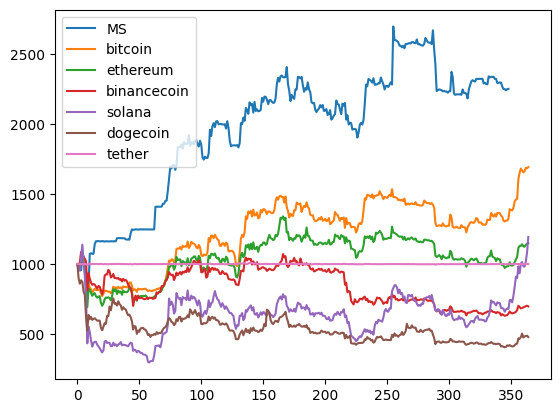
\includegraphics[scale=0.8]{./ms_with_tether.png}
	\caption{Comparison of the proposed model with single asset strategies.}
	\label{fig:versions}
\end{figure}

Moreover, Figure \ref{fig:changes1} depicts the behaviors of the optimal coin-switching strategy over the investment period. As shown in the figure, the strategy predominantly involves switching between coins when there are noticeable declines in coin prices, while minor price fluctuations have minimal impact on the agent's decisions.



\begin{figure}[h]
	\centering
	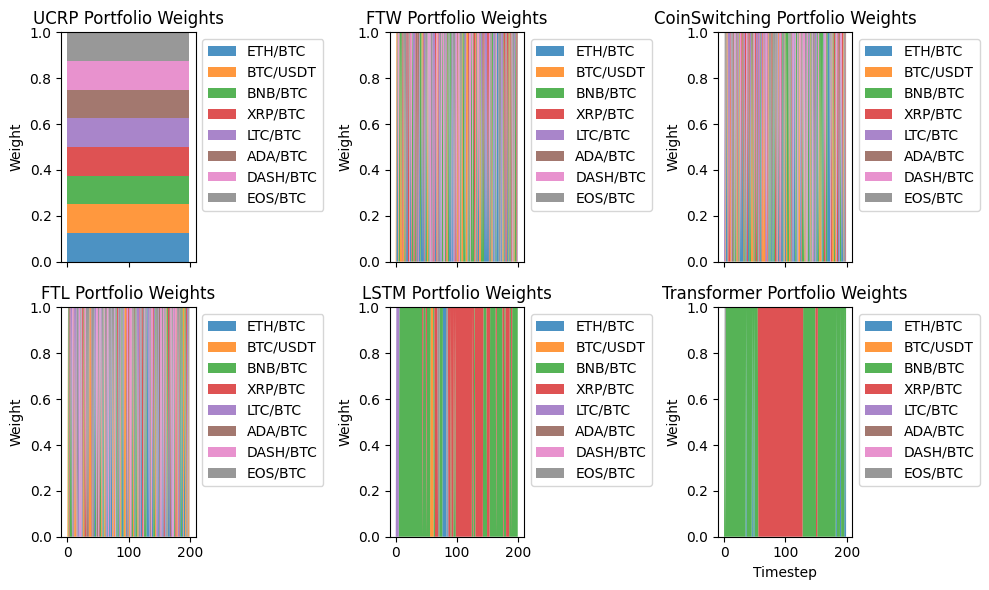
\includegraphics[scale=0.8]{./changes1.png}
	\caption{Model selection during investment timesteps}
	\label{fig:changes1}
\end{figure}

%
%\subsection{Comparison with Portfolio Management Strategies}
%
%
%In the final part of our experiments, we compare the performance of our proposed method with other state-of-the-art models for portfolio management in the cryptocurrencies market. We evaluate key metrics such as return on investment, Sharpe ratio, and maximum drawdown to assess the effectiveness and robustness of our approach in generating optimal stock portfolios under uncertainty. By benchmarking our method against existing models, we aim to demonstrate its superiority in handling volatility and risk in the crypto market.
%
%Through these experiments, we seek to validate the efficacy of our proposed method for stock portfolio management in the cryptocurrencies market and provide insights into its performance compared to alternative approaches. The results of these experiments will contribute to advancing AI-driven strategies for financial applications and enhancing decision-making processes in dynamic and unpredictable markets.
%
%
%
%
%\begin{figure}[h]
%	\centering
%	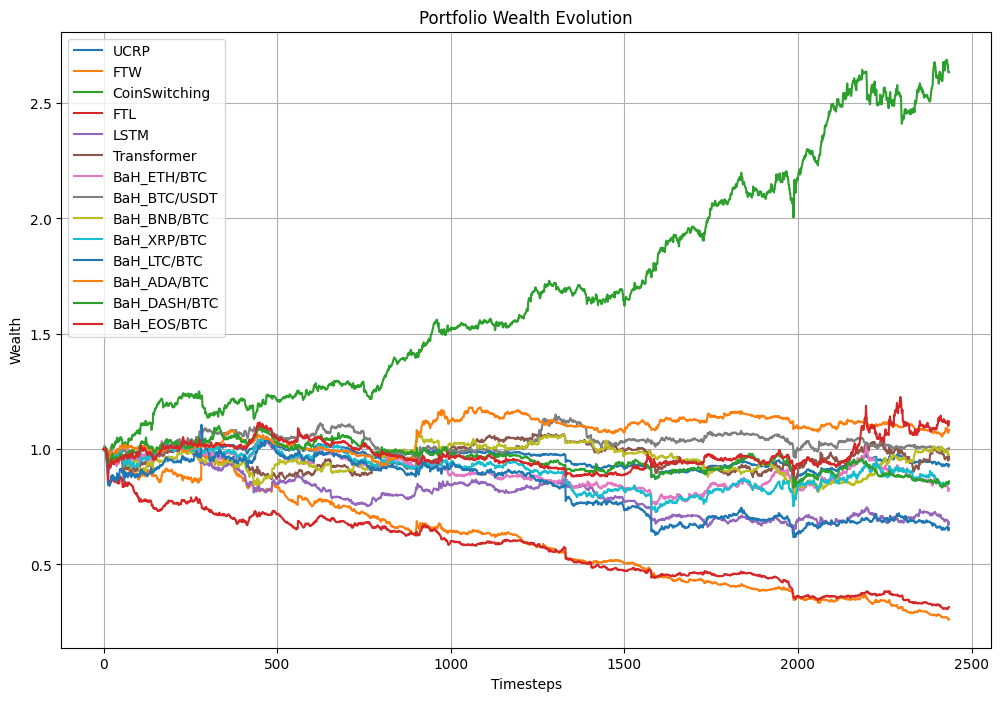
\includegraphics[scale=0.8]{./ms1.png}
%	\label{fig:ms1}
%	\caption{Model performance over coin performances during investment period}
%\end{figure}
%
%
%
%


\section{Conclusion}


In conclusion, the proposed model for stock portfolio management in the cryptocurrencies market demonstrates several key advantages and some limitations that are important to consider:

\subsection{Advantages}

\begin{enumerate}
	\item Effective uncertainty estimation: The integration of a Variational Autoencoder (VAE) enables our model to accurately quantify uncertainty in stock price predictions, providing valuable insights for risk management and decision-making.
	
	\item Dynamic portfolio optimization: The Actor-Critic neural network architecture allows for adaptive and dynamic portfolio rebalancing based on changing market conditions, leading to improved performance and resilience against volatility.
	
%	\item Robust Performance: Through extensive experimentation and comparison with state-of-the-art models, our method consistently achieves competitive results in terms of return on investment, Sharpe ratio, and maximum drawdown, showcasing its effectiveness in generating optimal stock portfolios.
	
	\item Real-world applicability: Leveraging a comprehensive dataset of historical cryptocurrency prices, our model operates under realistic market conditions, enhancing its practical relevance and applicability for financial institutions and investors.
	
\end{enumerate}


\subsection{Weaknesses}

\begin{enumerate}
%	\item Complexity: The complexity of the proposed model, particularly the integration of multiple neural network components and hyperparameters, may pose challenges in implementation and interpretation for users without a deep understanding of machine learning techniques.
	
	\item Data dependency: The performance of our model heavily relies on the quality and availability of historical asset price data during the training phase, which may limit its effectiveness in scenarios where data is scarce or unreliable.
	
%	\item Training Time: Training neural networks for portfolio optimization can be computationally intensive and time-consuming, especially when dealing with large datasets and complex architectures, potentially hindering real-time decision-making processes.
	
\end{enumerate}


Overall, the benefits of the proposed model outweigh its limitations, as it offers a data-driven approach to assess uncertainty of price trends in stock portfolio management in the volatile cryptocurrencies market. By addressing uncertainties and optimizing portfolios dynamically,giggg our method provides a valuable tool for investors seeking to navigate the complexities of cryptocurrency trading with enhanced confidence and efficiency. Further research and refinement of the model could help mitigate its limitations and unlock even greater potential for AI-driven financial strategies in the future.

\bibliographystyle{elsarticle-num-names} 
\bibliography{references}

%\section*{References}
%\bibliography{references}

%\appendix
%\input{Appendix}




\end{document}